\subsection{Multiclass Classification}
\label{subsec:multiclass}

Multiclass Classification is a problem of classifying the samples into several different classes and online learning is performed as a sequence of trials experiment. To solve this problem, the algorithms are aiming at learning a predictor $h: \mathscr{X} \rightarrow \mathscr{Y}$, which maps the instances to the classes space. The simplest approach to tackle multiclass prediction problem is by reduction from multiclass classification to binary classification. That is the methods we often mention: One-versus-All and All-versus-All. See Figure~\ref{pig:multiclass0}, there are some points classified into three classes (classified as their colors), by the method One vs All, it's necessary to find three binary classifiers who can only identify one class see Figure~\ref{pig:multiclass123}. Crammer has introduced several additive and multiplicative algorithms in \cite{crammer2003ultraconservative}, where Perceptron \cite{rosenblatt1958perceptron} and Winnow \cite{littlestone1988learning} are two such important algorithms. Much analysis has been done, Kivinen and Warmuth developed potential functions that can be used to analyze different online algorithm \cite{kivinen1995additive}. 

\begin{figure}[!h]
\vspace{.2in}
\centering{
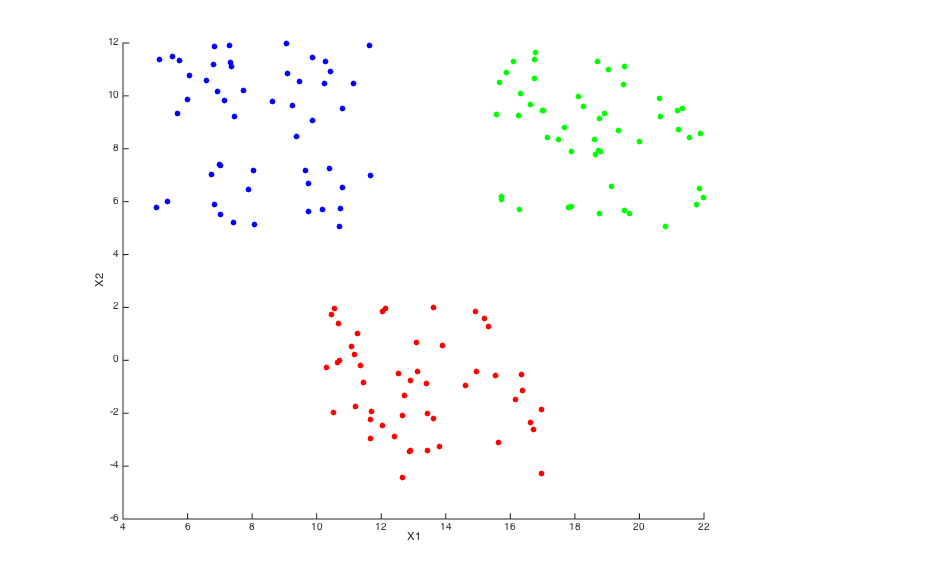
\includegraphics[scale = 0.5]{chapters/chapter03/fig03/mc/originalml.png}}
\caption{Multiclass task}
\label{pig:multiclass0}
\end{figure}

\begin{figure}[!h]
\vspace{.2in}
\centerline{
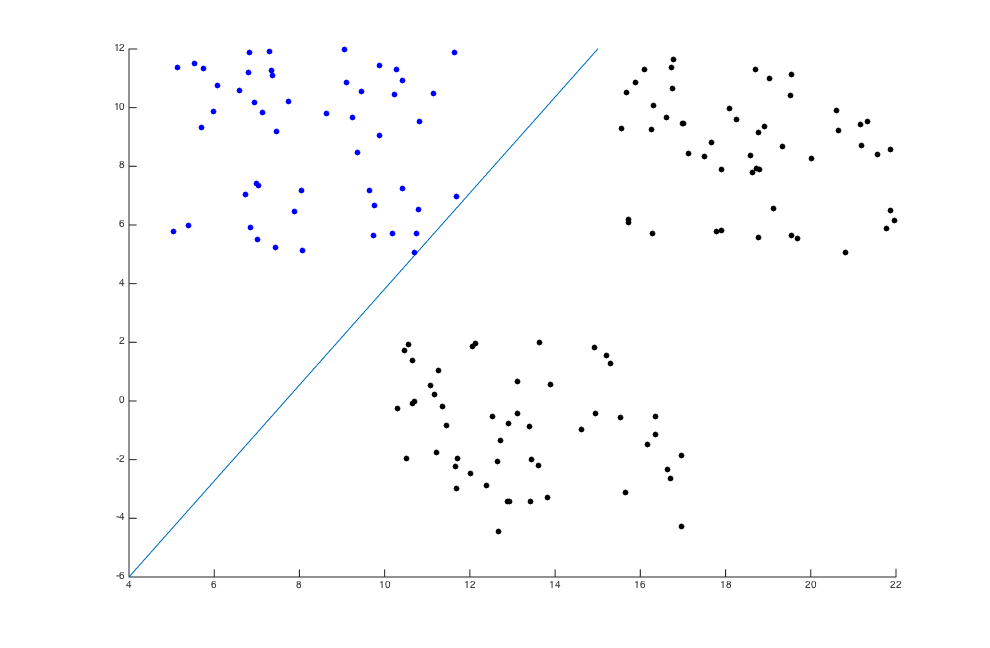
\includegraphics[width=0.6\linewidth]{chapters/chapter03/fig03/mc/class1.png}}
\centerline{
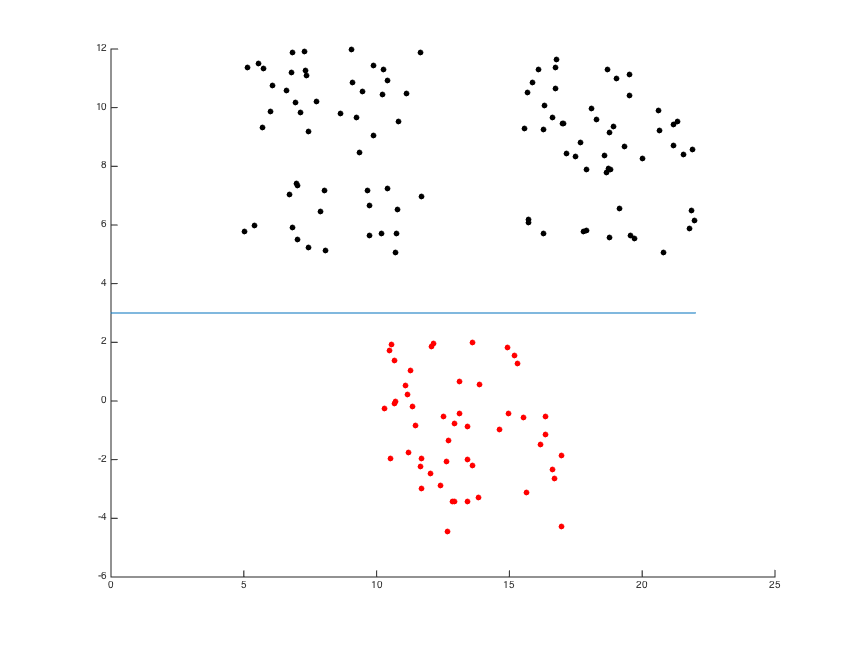
\includegraphics[width=0.6\linewidth]{chapters/chapter03/fig03/mc/class2.png}}
\centerline{
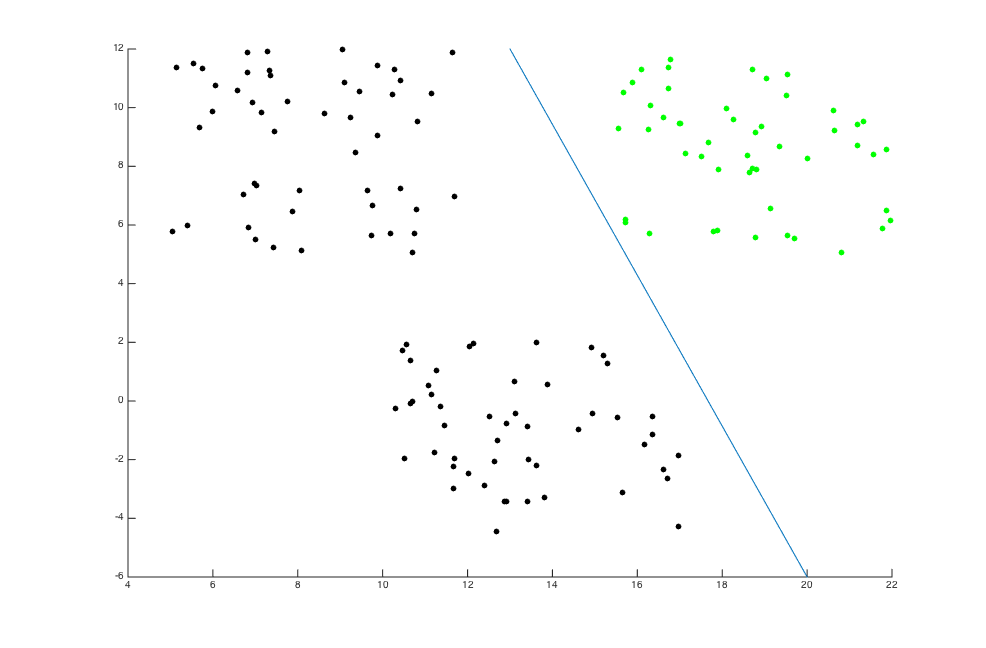
\includegraphics[width=0.6\linewidth]{chapters/chapter03/fig03/mc/class3.png}}
\caption{Reduction from multiclass classification to binary classification (One vs All)} 
\label{pig:multiclass123}
\end{figure}

For the process of multiclass classification online learning, at trial $t$, the algorithm firstly samples an instance $x_t \in \inputS\subseteq \Rd$ and classifies it into the set of all possible labels constitutes a finite set denoted by $\outputS$. Mostly, the algorithms of online classification assume that $\outputS$ is known in advance. We denote the set of unique labels observed on rounds from $1$ to $t-1$ by $Y_t$ ( In general, this set is known in advance and non-changeable during all rounds, so it could be simplified by $Y$). After predicted the label $\hy$ by the algorithm of online learning, the true class $y_t\in Y_t$ is revealed. Sometimes, the prediction $\hy$ is different to the true label $y_t$, in that case, it makes an incorrect prediction. To evaluate the accuracy or quality of classifiers, the prediction mistakes (denoted as $M$), regret (or instantaneous loss, as $l$) or cumulative regret (denoted as $R$ or $L$) come into being. To be computed on each round, specially when $\hy \neq y_t$.

The goal of all classification algorithms, is to minimize the total number of prediction mistakes or cumulative regret. To achieve this goal, the algorithms should update the classifiers by supervised learning mechanism at the end of each trial. 

Here, we make some definitions:  the feature vector representation $\pxy$ induced by the instance label pair $(\mathbf{x},y)$. Here, $\pxy$ is a $K\times d$ matrix which is composed of $K$ blocks of feature size $d$. All blocks but the $y$'th block of $\pxy$ are set to be the zero vector while the $y$'th blocks is set to be $\mathbf{x}$. Applying a single prototype multi-class algorithm to this problem produces a hypothesis $w \in \mathbb{R}^{K\times d}$ from $\mathscr{W}$ on every online round. Analogous to the construction of $\pxy$, $w$ is composed of $K$ blocks of size $d$ and denote block $r$ by $w_r$. By construction, we get that $<w \cdot \Phi(x_t,r) >= <w_r, x_t>$. Recall the hinge loss in binary classification, it's defined to be $[1-y_t<w,\xt>]_+$, where $[a]_+$ means $\text{max}(a,0)$. The hinge loss in the multiclass frame as follows:
\begin{equation}
\label{equa:hingelossML}
l(w_t;(\xt,y_t,\hy)) = [1+ <w_t, \Phi(\xt,\hy)> - <w_t, \Phi(\xt,y_t)>]_+
\end{equation}
After introduce the principal multiclass definitions, in the following of this section, we study some approaches for learning multiclass classifiers. Most of them are linear multiclass predictors. 

\vspace{3ex}
\textbf{Perceptron} was proposed by F. Rosenblatt \cite{rosenblatt1958perceptron}. It is a general computational model with some numerical weights. By Minsky and Papert \cite{minsky1987perceptrons}, it was refined and perfected in 1960s.  For the simplest binary model, the input space $\mathscr{X}\subseteq \mathbb{R}^d$ can be separated into two sets $P$ and $N$. The algorithm Perceptron is to look for a weight vector $w\in \mathbb{R}$ with a product function $h$, where $h(x_t) = <w,x_t> \in \mathbb{R}$. If the $P$ and $N$ are linear separated, the ideal weighted vector be assumed that all points of $P$ holds the product $h(x_P) > 0$ and all points of $N$ holds $h(x_N) < 0$. 

Generally, it initiates to choose the weight vector $w_0$ randomly. For the binary state, if the instance on round $t^{th}$ $x_t$ belongs to the set $P$,  $y_t$ the class of instance $x_t$ is $+1$, else $y_t$ equals to $-1$. Then, $y_t\cdot h(x_t) > 0$, it means the weight vector make a good prediction, and continue to predict a new instance; from the opposite direction, when it predicts wrong, the value of product $y_t \cdot h(x_t) <0$, it should take an update to the weight vector with the instance vector $x_t$
\[w_{t+1} = \begin{cases}
 w_t & \text{if } y_t \cdot h(x_t) >0\\ 
 w_t + y_t\cdot x_t & \text{else}
\end{cases} \]

The Perceptron in multiclass classification with $K$ classes, it should look for a set of $K$ weight vectors $W = (w_1,w_2,\dots,w_K) \in \mathscr{W} \subseteq \mathbb{R}^{K\times d}$. The prediction way should be referred to the Function~\ref{equa:prediction}. However, Perceptron updates according to the incorrect classification for each instance. It does not benefit the global information by its instantaneous strategy, so it is a greedy, local algorithm, and to be lead to an exponential number of updates with data non-separable. Its mistake bound convergence in $(R/\gamma)^2$ where $R = \text{max} \parallel{x_t}\parallel$ and $\gamma = \text{min} |<u,x_t>|$ with ideal classifiers $u$. More details of Perceptron see Appendix~\ref{algo:perceptron}.

\vspace{3ex}
\textbf{Second-order Perceptron}\cite{cesa2005second}. In the previous part, we talked about a popular, local and greedy linear algorithm-- Perceptron. Its serious problem is with incremental correlation. Here, we address a second order variant of Perceptron, which is proposed by Cesa-Bianchi. In this algorithm, there is a correlation matrix $S_t = \sum_{s=1}^t x_sx_s^T \in \mathbb{R}^{d\times d}$. With $S_t^{-1}$, the correlation matrix is reduced  to the identity matrix $I_t$.  

In the basic form, Second-order Perceptron algorithm takes an input parameter $a>0$. to compute its prediction in trial $t$ the algorithm uses an $d$-row matrix $S_{t-1}$ and an $K$-dimensional weight vector $w_{t-1}$, where subscript $t-1$ indicates the number of times matrix $S$ and vector $w$ have been updated in the first $t-1$ trials. Initially, the algorithm sets $S_0 = \mathbf{0}$ and $w_0 = \mathbf{0}$. Upon receiving the $t^{th}$ instance $x_t$, the algorithm  predicts the label of $x_t$ with $\hat{y}_t = \text{arg max}_{i\in\{1,\dots,K\}} \left((\sum_{s=1}^{t-1}y_t x_s)^T (a I_d+S_tS_t^T)^{-1}x_t\right)$, with $I_d$ being the $d\times d$ identity matrix. If $\hat{y}_t\neq y_t$, then a mistake occurs and the algorithm updates, if $\hat{y}_t = y_t$, no update takes place, and hence the algorithm is mistake driven. 

The second-order Perceptron algorithm retains the properties of sparsity and efficient dual variable representation. This allows us to efficiently run the algorithm in any reproducing Kernel Hillbert space for the non-linear situation.  By introducing the second-order matrix, Second Order Perceptron can effectively reduce the misclassification around the boundary and assumed to get a mistake upper bound. Confidence weighted can maintain each feature with a different confidence level, in order that the features with low degree of confidence need to update than the one with high level. To minimize KL divergence, the confidence weighted update method to ensure that the probability of each new sample can be correctly classified never be less than a fixed parameter. 

\vspace{3ex}
\textbf{Passive-Aggressive Algorithm}\cite{crammer2006online} is an effective framework for performing max-margin online learning.  Here, we address Online Passive-Aggressive algorithms, who learns the predictors from the linear hypothesis space during an online sequential. 

Here, all definitions are consistent with other sections. $\gamma\left(w_t;(x_t,y_t)\right)$ is used to present the margin between each labels.
\[\gamma\left(w_t;(x_t,y_t)\right)  = <w_t, \Phi(x_t,y_t)>-\underset{s\neq y_t}{max } <w_t\cdot \Phi(x_t,s)>\].

The margin is positive only if the relevant label is with higher density than all of the other irrelevant labels. With the definition of margin, it computes an instantaneous loss by hinge-loss function as following,
\begin{equation}
\label{equa:hingeloss}
l(w;(x,Y)) = 
\begin{cases}
0 & \gamma(w;(x,Y))\geqslant 1 \\ 
1-\gamma(w;(x,Y)) & \text{otherwise} 
\end{cases}
\end{equation}

The PA update rule is derived by defining the new weight $w_{t+1}$ as the solution to the optimization problem:
\begin{equation}
\label{equa:paconstraint}
w_{t+1} = \underset{w\in \mathbb{R}^d}{\text{argmin}} \frac{1}{2}\parallel{w-w_t}\parallel^2 \ \ s.t. \ \ \mathscr{l}(w;(x_t,Y_t)) = 0.
\end{equation}

Intuitively, if $w_t$ suffers no loss from the new instance, that the hinge loss $l_t(w_t;(\xt,y_t))$ equals to $0$, the algorithm passively assigns $w_{t+1} = w_t$; otherwise, it aggressively makes the new classifiers $w_{t+1}$ satisfy that $l_t(w_{t+1};(\xt,y_t))$ attain to no loss. 

The single constraint that choose to satisfy is $w\cdot\Phi(x_t,r_t)-w\cdot\Phi(x_t,s_t) \geqslant 1$ and thus $w_{t+1}$ is set to be the solution of the following simplified constrained optimization problem,
\begin{equation}
\label{equa:paoptimization}
w_{t+1} = \underset{w}{\text{argmin}}\frac{1}{2}\parallel{w-w_t}\parallel^2 \ \ s.t. \ \ w\cdot(\Phi(x_t,r_t)-\Phi(x_t,s_t))\geqslant 1
\end{equation}. 

The apparent benefit of this simplification lies in the fact that Eq.~\ref{equa:paoptimization} has a closed form solution. To draw the connection between the multilabel setting and binary classification,  considering of the vector $\Phi(x_t,y_t)-\Phi(x_t,\hy)$ as a virtual instance of a binary classification. Therefore, the closed form solution of Eq.~\ref{equa:paoptimization} is 
\begin{equation}
\label{equa:paupdate}
w_{t+1}=w_t +\tau_t \left( \Phi(x_t,y_t)-\Phi(x_t,\hy)\right)
\end{equation},
with,
\[\tau_t = \frac{l_t}{\parallel{\Phi(x_t,y_t)-\Phi(x_t,\hy)}\parallel^2}\]

Although it's essentially neglecting all but two labels on each step of the multiclass update, it can still obtain multiclass cumulative loss bounds. The key observation in the analysis it that,
\[l(w_t;(x_t,y_t)) = [<w_t,\Phi(x_t,y_t)-\Phi(x_t,\hy)>+1]_+\].

For the bounds of multiclass PA algorithm, it needs to cast the assumption that for all $t$ it holds that $\parallel{\Phi(x_t,y_t)-\Phi(x_t,\hy)}\parallel\leqslant R$ . This bound can immediately be converted into a bound on the norm of the feature set since $\parallel{\Phi(x_t,y_t)-\Phi(x_t,\hy)}\parallel \leqslant \parallel{\Phi(x_t,y_t)}+\parallel{\Phi(x_t,\hy)}\parallel$ . Thus, if the norm of the mapping $\Phi(x_t,k)$ is bounded for all $t$ and $k\in\mathscr{Y}$ then so is $\parallel{\Phi(x_t,y_t)-\Phi(x_t,\hy)}\parallel$ .  And the bounds on the cumulative loss of the algorithms is relative to the smallest loss that can be attained by any fixed hypothesis.